\documentclass[12pt, a4paper]{article}
\usepackage[margin=1in]{geometry}
\usepackage{graphicx}
\usepackage{amsmath}
\usepackage{xcolor}
\usepackage{tabularx}
\usepackage{booktabs}
\usepackage{listings}
\usepackage{tikz}
\usepackage{hyperref}
\usepackage{tocloft}
\usepackage{array}
\usepackage{makecell}
\usetikzlibrary{er, positioning, shapes.geometric, arrows.meta}

\definecolor{codegray}{rgb}{0.9,0.9,0.9}
\lstset{
    language=SQL,
    backgroundcolor=\color{codegray},
    basicstyle=\ttfamily\small,
    breaklines=true,
    frame=single,
    captionpos=b,
    keywordstyle=\color{blue}\bfseries,
    stringstyle=\color{red}
}

\begin{document}

% --- TITLE PAGE ---
\begin{titlepage}
    \centering
    \vspace*{1cm}
    
    {\Large \textbf{SVKM's NMIMS}} \\[0.4cm]
    {\Large \textbf{School of Technology Management \& Engineering, Indore}} \\[0.4cm]
    {\large \textbf{A.Y. 2025 -- 26}} \\[0.8cm]
    {\large \textbf{Course: Database Management Systems}} \\[1cm]
    
    \rule{\linewidth}{0.5pt} \\[0.5cm]
    {\Huge \textbf{Project Report}} \\[0.3cm]
    \rule{\linewidth}{0.5pt} \\[1cm]

    \begin{tabular}{@{} l l @{}}
        \textbf{Program:} & BTECH CE \\[4pt]
        \textbf{Semester:} & IV \\
    \end{tabular}

    \vspace{1cm}
    {\LARGE \textbf{CHAINVOTE -- E-VOTING SYSTEM}} \\[1.2cm]

    {\large \textbf{Details of Project Members}} \\[0.5cm]
    \begin{tabular}{|>{\centering\arraybackslash}p{2cm}|>{\centering\arraybackslash}p{2cm}|>{\centering\arraybackslash}p{6cm}|}
        \hline
        \textbf{Batch} & \textbf{Roll No.} & \textbf{Name} \\
        \hline
        B2 & F149 & Srishti Jain \\
        \hline
        B2 & F118 & Diksha Rathi \\
        \hline
        B2 & F061 & Tanay Trivedi \\
        \hline
    \end{tabular}

    \vspace{1cm}
    {\normalsize \textbf{Date of Submission:} 08/02/2026} \\[1cm]

    {\large \textbf{Contribution of Each Project Member}} \\[0.5cm]
    \begin{tabular}{|>{\centering\arraybackslash}p{2cm}|>{\centering\arraybackslash}p{3cm}|>{\raggedright\arraybackslash}p{7cm}|}
        \hline
        \textbf{Roll No.} & \textbf{Name} & \makecell[l]{\textbf{Contribution}} \\
        \hline
        F149 & Srishti Jain & Database Schema Design, Normalization, ER Modeling, and Core Logic \\[4pt]
        \hline
        F118 & Diksha Rathi & SQL Query Optimization, Joins, Triggers, and Constraints Setup \\[4pt]
        \hline
        F061 & Tanay Trivedi & Aggregation Queries, Backend Connection, System Integrations \\
        \hline
    \end{tabular}

    \vspace{1cm}
    \textbf{GitHub Link:} \url{https://github.com/chain-vote/chainvote/}
    \vspace{1cm}
    \newline
    \textbf{Deployed Link:} \url{https://chain-vote.onrender.com/}

\end{titlepage}

\newpage
\tableofcontents
\newpage

% --- I. STORYLINE ---
\section{Storyline}
ChainVote was conceived out of the necessity to construct an immutable, zero-trust digital election framework. By bridging the efficiency of traditional relational databases (like PostgreSQL/SQLite) with cryptographic Merkle tree hash-chaining, we overcome the ``Electronic Voting Paradox''. The chosen database topic aims to securely handle user identities, electoral candidates, real-time voting data, and cryptographic hashing while maintaining anonymity. The system uses a strict append-only mechanism. When a user casts a ballot, their vote is chained to the previous vote using SHA-256 hashes, structurally preventing arbitrary administrative mutation and ensuring complete systemic auditability.

% --- II. COMPONENTS OF DATABASE DESIGN ---
\section{Components of Database Design}
The database design ensures highly normalized relation structures augmented with cryptographic constraints.

\subsection{Entities and Attributes}
\begin{enumerate}
    \item \textbf{User (Voter)} \\
    \textit{Attributes:} \underline{\texttt{id}} (PK), \texttt{name}, \texttt{email}, \texttt{voterHash}, \texttt{isCommissioner}

    \item \textbf{Election} \\
    \textit{Attributes:} \underline{\texttt{id}} (PK), \texttt{title}, \texttt{status}, \texttt{merkleRoot}, \texttt{createdAt}

    \item \textbf{Candidate} \\
    \textit{Attributes:} \underline{\texttt{id}} (PK), \texttt{name}, \texttt{party}, \texttt{electionId} (FK)

    \item \textbf{Vote} \\
    \textit{Attributes:} \underline{\texttt{id}} (PK), \texttt{voterHash}, \texttt{electionId} (FK), \texttt{candidateId} (FK), \texttt{voteHash}, \texttt{prevHash}, \texttt{timestamp}
\end{enumerate}

\subsection{Relationships, Cardinality, and Participation}
\begin{itemize}
    \item \textbf{Election -- Candidate:} \textit{One-to-Many} (1:N). An election can have many candidates, but a candidate belongs to strictly one election. Total participation for Candidates.
    \item \textbf{Election -- Vote:} \textit{One-to-Many} (1:N). An election logs multiple votes. Total participation for Votes.
    \item \textbf{Candidate -- Vote:} \textit{One-to-Many} (1:N). A candidate receives multiple votes.
    \item \textbf{User -- Vote (Conceptual):} There is technically no physical Foreign Key from \texttt{User} to \texttt{Vote} on purpose to maintain anonymity; instead linked via one-way \texttt{voterHash}.
\end{itemize}

\newpage
% --- III. ENTITY RELATIONSHIP DIAGRAM ---
\section{Entity Relationship Diagram}

\begin{center}
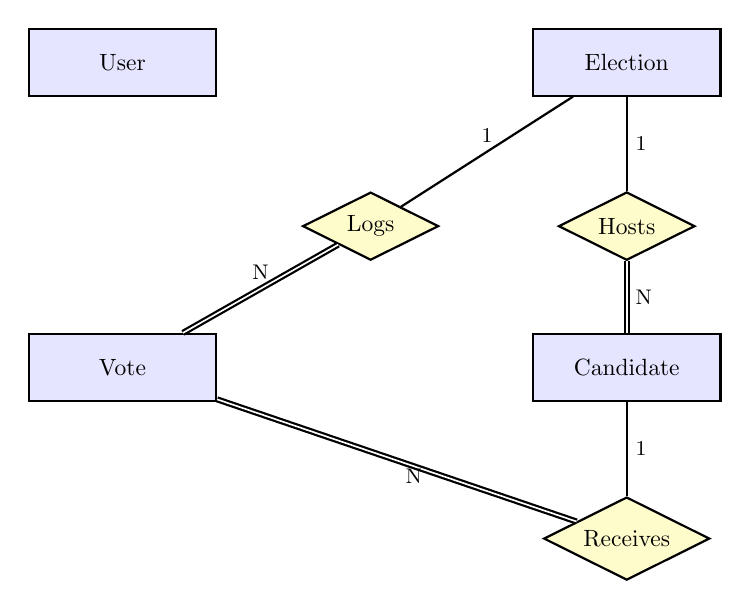
\begin{tikzpicture}[
    node distance=3cm,
    entity/.style={rectangle, draw=black, thick, minimum width=2.8cm, minimum height=1cm, fill=blue!10, align=center},
    relation/.style={diamond, draw=black, thick, fill=yellow!20, aspect=2, align=center},
    every node/.style={scale=0.85}
]

    % Entities
    \node[entity] (Election)   {Election};
    \node[entity] (Candidate)  [below=3cm of Election] {Candidate};
    \node[entity] (Vote)       [left=4cm of Candidate] {Vote};
    \node[entity] (User)       [left=4cm of Election]  {User};

    % Relationships
    \node[relation] (Hosts)    [below=1.2cm of Election]  {Hosts};
    \node[relation] (Logs)     [left=1.5cm of Hosts]      {Logs};
    \node[relation] (Receives) [below=1.2cm of Candidate] {Receives};

    % Edges
    \draw[thick] (Election)  -- node[right, font=\small] {1} (Hosts);
    \draw[thick, double] (Hosts) -- node[right, font=\small] {N} (Candidate);

    \draw[thick] (Election)  -- node[above, font=\small] {1} (Logs);
    \draw[thick, double] (Logs) -- node[above, font=\small] {N} (Vote);

    \draw[thick] (Candidate) -- node[right, font=\small] {1} (Receives);
    \draw[thick, double] (Receives) -- node[below right, font=\small] {N} (Vote);

\end{tikzpicture}
\end{center}

% --- IV. RELATIONAL MODEL ---
\section{Relational Model}
Based on the ER diagram, the relational schemas are established as follows:

\begin{itemize}
    \item \textbf{Users}\,(\underline{id}, name, email, voterHash, isCommissioner)
    \item \textbf{Election}\,(\underline{id}, title, status, merkleRoot, createdAt)
    \item \textbf{Candidate}\,(\underline{id}, name, party, \textit{electionId}) \\
          \hspace*{1em}\textit{Foreign Key:} \texttt{electionId} $\to$ \texttt{Election(id)}
    \item \textbf{Vote}\,(\underline{id}, voterHash, \textit{electionId}, \textit{candidateId}, voteHash, prevHash, timestamp) \\
          \hspace*{1em}\textit{Foreign Key:} \texttt{electionId} $\to$ \texttt{Election(id)} \\
          \hspace*{1em}\textit{Foreign Key:} \texttt{candidateId} $\to$ \texttt{Candidate(id)} \\
          \hspace*{1em}\textit{Unique Constraint:} \texttt{(voterHash, electionId)}
\end{itemize}

% --- V. NORMALIZATION ---
\section{Normalization}

\begin{description}
    \item[\textbf{1NF:}] All attributes are atomic. The schema avoids multi-valued attributes such as multiple emails per row.
    \item[\textbf{2NF:}] All relations are in 1NF and every non-prime attribute is fully functionally dependent on the primary key. Since primary keys are single atomic UUIDs, there are no partial dependencies.
    \item[\textbf{3NF:}] All relations are in 2NF with no transitive dependencies. For example, \texttt{party} depends only on \texttt{Candidate(id)}, not on \texttt{name}.
    \item[\textbf{BCNF:}] For every functional dependency $X \rightarrow Y$, $X$ is a superkey. Our system satisfies this natively.
\end{description}

\newpage
% --- VI. SQL QUERIES ---
\section{SQL Queries}

\subsection{1.\ Create Users Table}
\textbf{Question:} Create the table \texttt{Users} with a unique email and voterHash.
\begin{lstlisting}
CREATE TABLE Users (
    id            VARCHAR(50)  PRIMARY KEY,
    name          VARCHAR(100),
    email         VARCHAR(100) UNIQUE,
    voterHash     VARCHAR(64)  UNIQUE,
    isCommissioner BOOLEAN      DEFAULT FALSE
);
\end{lstlisting}

\subsection{2.\ Create Election Table}
\textbf{Question:} Create the \texttt{Election} table storing the Merkle Root.
\begin{lstlisting}
CREATE TABLE Election (
    id         VARCHAR(50)  PRIMARY KEY,
    title      VARCHAR(150),
    status     VARCHAR(20),
    merkleRoot VARCHAR(64),
    createdAt  DATETIME     DEFAULT CURRENT_TIMESTAMP
);
\end{lstlisting}

\subsection{3.\ Create Candidate Table}
\textbf{Question:} Create the \texttt{Candidate} table with a foreign key referencing \texttt{Election}.
\begin{lstlisting}
CREATE TABLE Candidate (
    id         VARCHAR(50)  PRIMARY KEY,
    name       VARCHAR(100),
    party      VARCHAR(100),
    electionId VARCHAR(50),
    FOREIGN KEY (electionId) REFERENCES Election(id)
);
\end{lstlisting}

\subsection{4.\ Create Vote Table}
\textbf{Question:} Create the cryptographic \texttt{Vote} table ensuring a single vote per user per election.
\begin{lstlisting}
CREATE TABLE Vote (
    id          VARCHAR(50) PRIMARY KEY,
    voterHash   VARCHAR(64),
    electionId  VARCHAR(50),
    candidateId VARCHAR(50),
    voteHash    VARCHAR(64),
    prevHash    VARCHAR(64),
    timestamp   DATETIME    DEFAULT CURRENT_TIMESTAMP,
    FOREIGN KEY (electionId)  REFERENCES Election(id),
    FOREIGN KEY (candidateId) REFERENCES Candidate(id),
    UNIQUE (voterHash, electionId)
);
\end{lstlisting}

\subsection{5.\ Populate Users}
\textbf{Question:} Insert meaningful data into the \texttt{Users} table.
\begin{lstlisting}
INSERT INTO Users (id, name, email, voterHash, isCommissioner) VALUES
  ('u1', 'Srishti Jain',  'sj@example.com',    'hashA', TRUE),
  ('u2', 'Diksha Rathi',  'dr@example.com',    'hashB', FALSE),
  ('u3', 'Tanay Trivedi', 'tt@example.com',    'hashC', FALSE),
  ('u4', 'Alice Smith',   'alice@example.com', 'hashD', FALSE),
  ('u5', 'Bob Jones',     'bob@example.com',   'hashE', FALSE);
\end{lstlisting}

\begin{center}
\begin{tabular}{|>{\ttfamily}l|l|l|>{\ttfamily}l|c|}
\hline
\textbf{id} & \textbf{name} & \textbf{email} & \textbf{voterHash} & \textbf{isCommissioner} \\
\hline
u1 & Srishti Jain & sj@example.com & hashA & 1 \\
u2 & Diksha Rathi & dr@example.com & hashB & 0 \\
\ldots & \ldots & \ldots & \ldots & \ldots \\
\hline
\end{tabular}
\end{center}

\subsection{6.\ Populate Election and Candidates}
\textbf{Question:} Insert data into \texttt{Election} and \texttt{Candidate} tables.
\begin{lstlisting}
INSERT INTO Election (id, title, status) VALUES
  ('e1', 'General Election 2026', 'LIVE'),
  ('e2', 'Student Council 2026',  'DRAFT');

INSERT INTO Candidate (id, name, party, electionId) VALUES
  ('c1', 'John Doe',    'Progressive', 'e1'),
  ('c2', 'Jane Roe',    'Conservative','e1'),
  ('c3', 'Alan Turing', 'Tech Front',  'e2');
\end{lstlisting}

\begin{center}
\begin{tabular}{|>{\ttfamily}l|l|l|>{\ttfamily}l|}
\hline
\textbf{id} & \textbf{name} & \textbf{party} & \textbf{electionId} \\
\hline
c1 & John Doe & Progressive  & e1 \\
c2 & Jane Roe & Conservative & e1 \\
\hline
\end{tabular}
\end{center}

\subsection{7.\ Populate Votes}
\textbf{Question:} Record votes ensuring hash sequencing.
\begin{lstlisting}
INSERT INTO Vote (id, voterHash, electionId, candidateId, voteHash, prevHash)
VALUES
  ('v1', 'hashB', 'e1', 'c1', 'abcd123', NULL),
  ('v2', 'hashC', 'e1', 'c2', 'efgh456', 'abcd123'),
  ('v3', 'hashD', 'e1', 'c1', 'ijkl789', 'efgh456'),
  ('v4', 'hashE', 'e1', 'c1', 'mnop012', 'ijkl789');
\end{lstlisting}

\begin{center}
\begin{tabular}{|>{\ttfamily}l|>{\ttfamily}l|>{\ttfamily}l|>{\ttfamily}l|}
\hline
\textbf{id} & \textbf{voterHash} & \textbf{voteHash} & \textbf{prevHash} \\
\hline
v1 & hashB & abcd123 & NULL     \\
v2 & hashC & efgh456 & abcd123  \\
\hline
\end{tabular}
\end{center}

\subsection{8.\ Basic SELECT Query}
\textbf{Question:} Retrieve all live elections.
\begin{lstlisting}
SELECT title, status FROM Election WHERE status = 'LIVE';
\end{lstlisting}
\begin{center}
\begin{tabular}{|l|l|}
\hline
\textbf{title} & \textbf{status} \\ \hline
General Election 2026 & LIVE \\ \hline
\end{tabular}
\end{center}

\subsection{9.\ Update Query}
\textbf{Question:} Change the status of election \texttt{e2} to \texttt{LIVE}.
\begin{lstlisting}
UPDATE Election SET status = 'LIVE' WHERE id = 'e2';
\end{lstlisting}
\begin{center}
\begin{tabular}{|l|}
\hline
(1 row affected) \\ \hline
\end{tabular}
\end{center}

\subsection{10.\ Inner Join}
\textbf{Question:} Find the names of candidates and the election they belong to.
\begin{lstlisting}
SELECT c.name, e.title
FROM   Candidate c
INNER JOIN Election e ON c.electionId = e.id;
\end{lstlisting}
\begin{center}
\begin{tabular}{|l|l|}
\hline
\textbf{name} & \textbf{title} \\ \hline
John Doe    & General Election 2026 \\
Jane Roe    & General Election 2026 \\
Alan Turing & Student Council 2026  \\ \hline
\end{tabular}
\end{center}

\subsection{11.\ Aggregate Function: COUNT}
\textbf{Question:} Count the total number of votes cast in election \texttt{e1}.
\begin{lstlisting}
SELECT COUNT(id) AS total_votes FROM Vote WHERE electionId = 'e1';
\end{lstlisting}
\begin{center}
\begin{tabular}{|c|}
\hline
\textbf{total\_votes} \\ \hline
4 \\ \hline
\end{tabular}
\end{center}

\subsection{12.\ Group By with COUNT}
\textbf{Question:} Tally the votes for each candidate in election \texttt{e1}.
\begin{lstlisting}
SELECT candidateId, COUNT(*) AS VoteCount
FROM   Vote
WHERE  electionId = 'e1'
GROUP BY candidateId;
\end{lstlisting}
\begin{center}
\begin{tabular}{|>{\ttfamily}l|c|}
\hline
\textbf{candidateId} & \textbf{VoteCount} \\ \hline
c1 & 3 \\
c2 & 1 \\ \hline
\end{tabular}
\end{center}

\subsection{13.\ Order By Clause}
\textbf{Question:} Display votes in reverse chronological order.
\begin{lstlisting}
SELECT id, voteHash FROM Vote ORDER BY timestamp DESC;
\end{lstlisting}
\begin{center}
\begin{tabular}{|>{\ttfamily}l|>{\ttfamily}l|}
\hline
\textbf{id} & \textbf{voteHash} \\ \hline
v4 & mnop012 \\
v3 & ijkl789 \\
\ldots & \ldots \\ \hline
\end{tabular}
\end{center}

\subsection{14.\ Nested Query / Subquery}
\textbf{Question:} Find the name of the candidate who received the first vote.
\begin{lstlisting}
SELECT name FROM Candidate
WHERE id = (SELECT candidateId FROM Vote WHERE prevHash IS NULL);
\end{lstlisting}
\begin{center}
\begin{tabular}{|l|}
\hline
\textbf{name} \\ \hline
John Doe \\ \hline
\end{tabular}
\end{center}

\subsection{15.\ Join with Subquery}
\textbf{Question:} Retrieve candidate names and their total received votes.
\begin{lstlisting}
SELECT c.name, COUNT(v.id) AS total
FROM   Candidate c
LEFT JOIN Vote v ON c.id = v.candidateId
GROUP BY c.name;
\end{lstlisting}
\begin{center}
\begin{tabular}{|l|c|}
\hline
\textbf{name} & \textbf{total} \\ \hline
John Doe    & 3 \\
Jane Roe    & 1 \\
Alan Turing & 0 \\ \hline
\end{tabular}
\end{center}

\subsection{16.\ Having Clause}
\textbf{Question:} Find candidates who received more than 2 votes.
\begin{lstlisting}
SELECT candidateId, COUNT(id) AS VoteCount
FROM   Vote
GROUP BY candidateId
HAVING COUNT(id) > 2;
\end{lstlisting}
\begin{center}
\begin{tabular}{|>{\ttfamily}l|c|}
\hline
\textbf{candidateId} & \textbf{VoteCount} \\ \hline
c1 & 3 \\ \hline
\end{tabular}
\end{center}

\subsection{17.\ IN Operator}
\textbf{Question:} Find all voters who voted for candidate \texttt{c1} or \texttt{c2}.
\begin{lstlisting}
SELECT voterHash FROM Vote WHERE candidateId IN ('c1', 'c2');
\end{lstlisting}
\begin{center}
\begin{tabular}{|>{\ttfamily}l|}
\hline
\textbf{voterHash} \\ \hline
hashB \\ hashC \\ hashD \\ hashE \\ \hline
\end{tabular}
\end{center}

\subsection{18.\ LIKE Operator}
\textbf{Question:} Find all users with an \texttt{@example.com} email address.
\begin{lstlisting}
SELECT email FROM Users WHERE email LIKE '%@example.com';
\end{lstlisting}
\begin{center}
\begin{tabular}{|l|}
\hline
\textbf{email} \\ \hline
sj@example.com \\
dr@example.com \\
\ldots \\ \hline
\end{tabular}
\end{center}

\subsection{19.\ EXISTS Clause}
\textbf{Question:} Verify if any election has zero candidates.
\begin{lstlisting}
SELECT title FROM Election e
WHERE NOT EXISTS (
    SELECT 1 FROM Candidate c WHERE c.electionId = e.id
);
\end{lstlisting}
\begin{center}
\begin{tabular}{|l|}
\hline
\textbf{title} \\ \hline
(0 rows returned) \\ \hline
\end{tabular}
\end{center}

\subsection{20.\ Create a VIEW}
\textbf{Question:} Create a view representing the live election tally.
\begin{lstlisting}
CREATE VIEW ElectionTally AS
SELECT c.name, c.party, COUNT(v.id) AS Tally
FROM   Candidate c
LEFT JOIN Vote v ON c.id = v.candidateId
GROUP BY c.id;

SELECT * FROM ElectionTally;
\end{lstlisting}
\begin{center}
\begin{tabular}{|l|l|c|}
\hline
\textbf{name} & \textbf{party} & \textbf{Tally} \\ \hline
John Doe    & Progressive  & 3 \\
Jane Roe    & Conservative & 1 \\
Alan Turing & Tech Front   & 0 \\ \hline
\end{tabular}
\end{center}

% --- VII. PROJECT DEMONSTRATION ---
\section{Project Demonstration}

\textbf{Tools / Software / Libraries Used:}
\begin{itemize}
    \item \textbf{Frontend:} React, Vite, TailwindCSS, Three.js (Merkle visualisation)
    \item \textbf{Backend:} Node.js, Express, Socket.IO
    \item \textbf{Database:} SQLite / PostgreSQL via Prisma ORM
    \item \textbf{Cryptography:} SHA-256 for chain validations
\end{itemize}

\textbf{Description of Demonstration:} The application GUI features a dynamic Admin Dashboard (``Database Engine'') functioning natively as an SQL Workbench. It enables the Commissioner to run direct database queries securely. The ``Hall of Silence'' interface serves as the voting terminal ensuring anonymised ballot casting.

% --- VIII. SELF LEARNING ---
\section{Self-Learning Beyond Classroom}
During execution of this project, we explored advanced concepts well beyond the standard DBMS curriculum:
\begin{itemize}
    \item \textbf{Cryptographic Hashing in SQL:} Storing and maintaining SHA-256 sequences across dependent rows directly inside relational tables.
    \item \textbf{Object-Relational Mapping (ORM):} Moving beyond raw SQL, we integrated \texttt{Prisma ORM} to define schemas as code and perform type-safe database migrations.
    \item \textbf{Optimistic Database Concurrency:} Handling race conditions using \texttt{UNIQUE} constraints to deflect concurrent Sybil attacks.
\end{itemize}

% --- IX. LEARNING FROM THE PROJECT ---
\section{Learning from the Project}
This project cemented our understanding of relational algebra, the critical importance of normalization, and strict primary/foreign key mappings. Implementing the \texttt{UNIQUE(voterHash, electionId)} constraint demonstrated how business rules (one vote per person) are enforced at the database level rather than solely at the application layer.

% --- X. CHALLENGES FACED ---
\section{Challenges Faced}
\begin{itemize}
    \item \textbf{Cryptographic Chain Maintenance:} Devising a schema that inherently links \texttt{prevHash} across records and handles fork-collisions gracefully.
    \item \textbf{Anonymising Data:} Ensuring a user logged a vote (to prevent double-voting) while strictly decoupling their identity (\texttt{email}/\texttt{name}) from their chosen candidate -- solved via one-way detached \texttt{voterHash}.
\end{itemize}

% --- XI. CONCLUSION ---
\section{Conclusion}
ChainVote successfully demonstrates that complex, ultra-secure architectures can be elegantly built atop traditional relational DBMS models. The integration of 4-tier normalization, strict declarative constraints, and hash-chaining creates an immutable post-trust system -- a cornerstone representation of robust database design applied to modern cryptographic problems.

\end{document}